\subsection{Progettazione di Dettaglio e Codifica}
\label{progettazione_di_dettaglio}
\textbf{Durata:} dal 2021\_03\_09 al 2021\_04\_02 \\
Il periodo inizia appena concluso il precedente e termina con la \textbf{Revisione di Qualifica}. 

Le precondizioni sono:
\begin{itemize}
    \item Le postcondizioni del periodo precedente sono state soddisfatte.
\end{itemize}

Le postcondizioni sono:
\begin{itemize}
    \item Aggiornamento e correzione dei documenti già prodotti;
    \item Realizzazione dei diagrammi delle classi e delle attività;
    \item Completamento codifica e relativa verifica;
    \item Redazione manuale utente e manuale sviluppatore;
    \item Consegna dei documenti richiesti in entrata alla \textbf{Revisione di Qualifica};
    \item Ultimata preparazione della presentazione da esporre in sede di revisione.
\end{itemize}
È composto da nuovi incrementi e nuove attività:

\begin{itemize}
    \item \textbf{Incremento e Verifica dei documenti:} i documenti già prodotti vengono migliorati e aggiornati se necessario (\textit{\NdP}, \textit{\PdP}, \textit{Glossario},\textit{\PdQ}, \textit{\AdR}); 
    \item \textbf{Incremento e Verifica delle Attività}: Viene migliorata l'attività di \textit{Technology Baseline}), ampliando lo studio delle tecnologie mancanti e progettando ad alto livello come realizzare il prodotto finale.
    \item \textbf{Product Baseline:} Segue la \textit{Technology Baseline} ed è formata da 3 incrementi fondamentali per la codifica:
        \begin{itemize}
            \item \textbf{Design Pattern}: Vengono individuati e discussi in modo da capire quali siano necessari e come riuscire a integrarli al meglio nel progetto;
            \item \textbf{Diagrammi Classi}: Dopo un'attenta riflessione sul codice vengono realizzati i diagrammi delle classi;
            \item \textbf{Diagrammi Attività}: Dopo un'attenta riflessione sul codice vengono realizzati i diagrammi delle attività. 
        \end{itemize} 
    \item \textbf{Specifica Tecnica:} Viene realizzato un documento contenente tutte le caratteristiche del prodotto e le motivazioni che hanno portato alla loro scelta;
    \item \textbf{Codifica:} Viene scritto il codice con relativa verifica. Questa attività, dato il modello di sviluppo scelto, verrà suddivisa in incrementi che verranno definiti dopo aver preparato il \textit{Proof of Concept} così da avere una maggiore conoscenza sul lavoro effettivo da svolgere e poter progettare al meglio i vari incrementi.  
    \item \textbf{Manuale Utente:} Viene redatto un documento che indica le istruzioni d'uso specifico per l'utente.
\end{itemize}

\newpage
\subsubsection{Diagramma di Gantt: Progettazione di Dettaglio e Codifica}
\begin{figure}[ht]
    \centering
    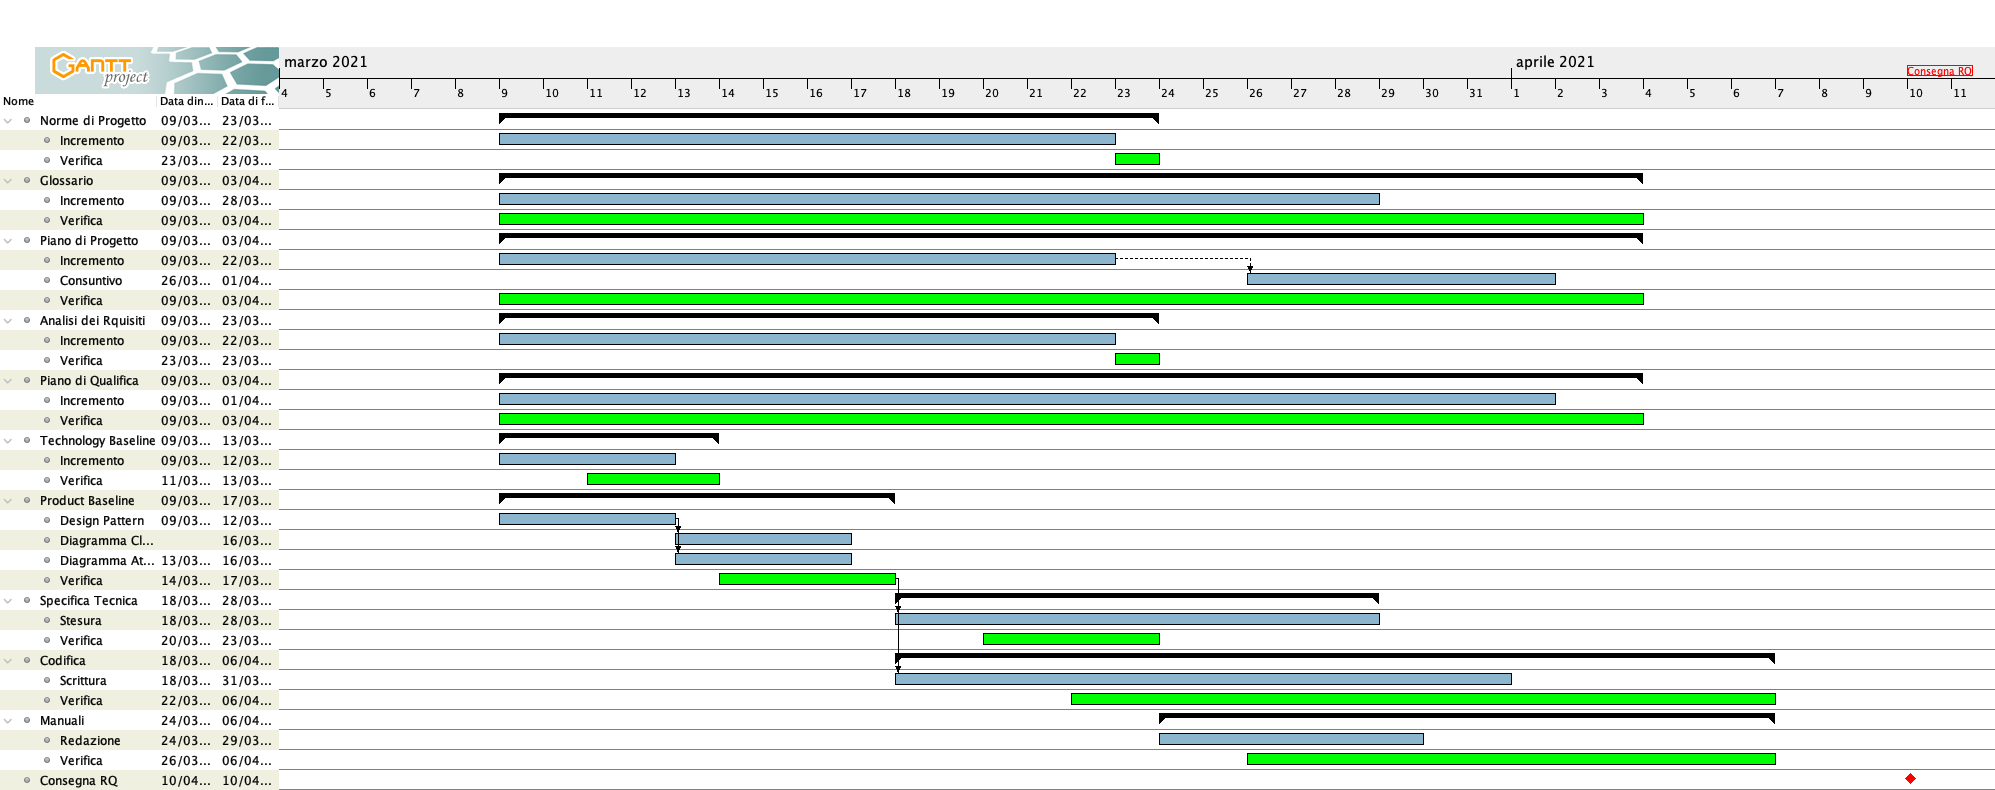
\includegraphics[width=\textwidth]{Immagini/GanttProgettazioneDiDettaglioECodifica}
    \caption{Diagramma di Gantt dell'attività di Progettazione di Dettaglio e Codifica}
\end{figure}